\section{Differenzierbare Funktionen}
\Def[4.1] Sei \( D \subseteq \R , f: D \rightarrow \R \) und \(x_0 \in D\) ein Häufungspunkt von D \newline
f ist ist \textbf{in \(x_0\) Differenzierbar}, falls der Grenzwert
\[ \lim\limits_{x \rightarrow x_0} \frac{f(x) - f(x_0)}{x - x_0}\]
existiert. Ist dies der Fall, wird der Grenzwert mit \(f'(x_0)\) bezeichnet \newline
\Bem{4.2}: Es ist oft von Vorteil in der Definiton von \(f'(x_0)\), \(x = x_0 +h\) zu setzen \[f'(x_0) = \lim_{h \rightarrow 0} \frac{f(x_0+h)-f(x_0)}{h}\]
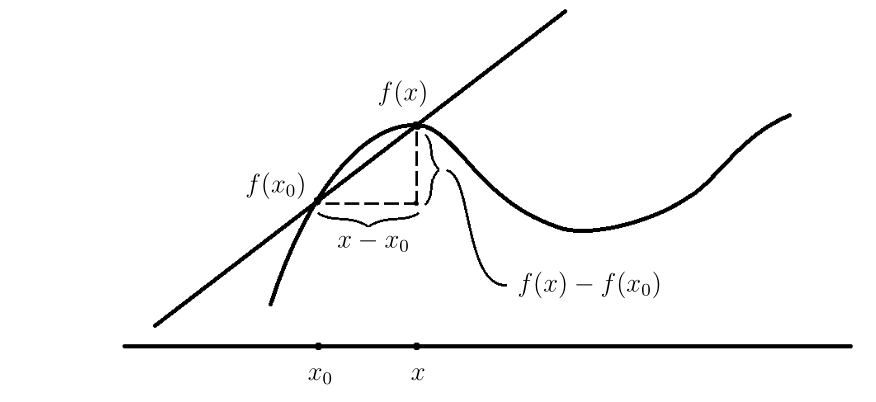
\includegraphics[scale=0.225]{differenzierbar.png} \newline
\( \frac{f(x) - f(x_0)}{x - x_0}\) ist die Steigung der Gerade durch \((x_0, f(x_0)), (x,f(x))\). Falls \(f'(x_0)\) existiert ist die Intuition, dass die Familien der Geraden durch \((x_0, f(x_0)), (x,f(x))\) für \(x \neq x_0, x \rightarrow x_0\) als "Grenzwert" die Tangente zum Graphen von f in \((x_0, f(x_0))\) annimmt.
\subsection{Die Ableitung}
\Satz[4.3](Weierstrass 1861). Sei \(f: D \rightarrow \R, x_0 \in D\) Häufungspunkt von D. Folgende Aussagen sind äquivalent:
\begin{enumerate}
    \item [1] f ist in \(x_0\) differenzierbar.
    \item [2] Es gibt \(c \in \R \) und \(r: D \rightarrow D \) mit:
    \begin{enumerate}
        \item  [2.1] \(f(x) = f(x_0) + c(x - x_0) + r(x)(x-x_0)\)
        \item  [2.2] \(r(x_0) = 0 \) und r ist stetig in \(x_0\)
    \end{enumerate} 
\end{enumerate}
Falls dies zutrifft ist \(c = f'(x_0)\) eindeutig bestimmt
Die Formulierung der Differenzierbarkeit von f mittels
\[ f(x) = f(x_0) + f'(x_0)(x - x_0) + r(x)(x - x_0)\]
und der Stetigkeit von r in \(x_0\) hat den Vorteil, dass sie keinen Limes enthält. Ausserdem ist dann
\[ y = f(x_0) + f'(x_0)(x - x_0)\]
die Gleichung der Tangente zum Graphen von f im Punkt \( (x_0, f(x_0))\).
WIr können die Charakterisierung der Differenzierbarkeit noch vereinfachen in dem wir in Satz 4.3(2.1)
\[ \phi(x) = f'(x_0) + r(x)\]
setzen. Wir erhalten: \newline
\Satz[4.4]Eine Funktion \( f: D \rightarrow \R\) ist genau dann in \(x_0\) differenzierbar, falls es eine Funktion \(\phi : D \rightarrow \R \) gibt die stetig in \(x_0\) ist und so, dass
\[f(x) = f(x_0) + \phi(x)(x - x_0) \quad \forall x \in D\]
In diesem Fall gilt \(\phi(x_0) = f'(x_0)\) \newline
\Korollar[4.5] Sei \(f : D \rightarrow \R \) und \(x_0 \in D \) ein Häufungspunkt von D. Falls \(f\) in \(x_0\) differenzierbar ist, so ist \(f\) stetig in \(x_0\) \newline
\Bsp[4.6] \begin{enumerate}
    \item  \( f = 1: \R \rightarrow \R\), dann ist \(f'(x) = 0 \quad  \forall x_0 \in \R \)
    Folgt aus \(f(x) - f(x_0) = 1 - 1 = 0\)
    \item  \( f : \R \rightarrow \R, f(x) = x\). Dann ist \(f'(x_0)=1\) \newline
    Folgt aus \(f(x) - f(x_0) = 1 \cdot (x - x_0) \)
    \item  \(f: \R \rightarrow \R, f(x) = x^2\). Dann ist \(f'(x_0) = 2x_0 \quad \forall x_0 \in \R\) \newline
    Folgt aus:
    \[ f(x) - f(x_0) = x^2 - x_0^2 = (x-x_0)(x+x_0)\]
    Also für \( x \neq x_0:\)
    \[ \frac{f(x) - f(x_0)}{x - x_0} = x + x_0\]
    woraus
    \[ \lim_{x \rightarrow x_0} \frac{f(x) - f(x_0)}{x - x_0} = \lim_{x \rightarrow x_0} (x + x_0) = 2x_0\]
    folgt.
    \item  \(f: \R \rightarrow \R, f(x) = \abs{x}\) \newline
    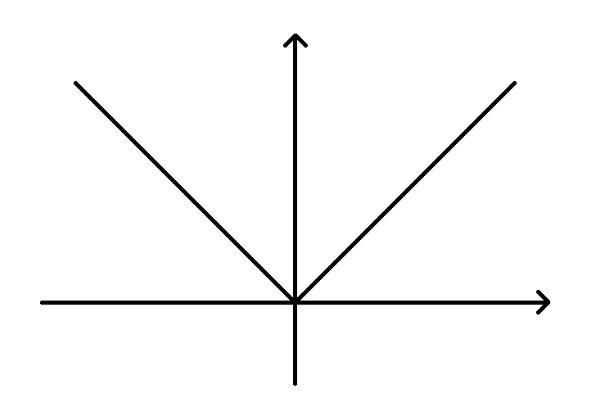
\includegraphics[scale=0.225]{ABS-function.png}
    \newline
    Ist in \(x_0 = 0\) nicht differenzierbar: \newline
    Für \( x < 0:\)
    \[ \frac{f(x) - f(0)}{x - 0} = \frac{\abs{x}}{x} = -1\]
    Für \( x > 0:\)
    \[ \frac{f(x) - f(0)}{x - 0} = \frac{\abs{x}}{x} = 1\]
    Also hat für \(x \rightarrow 0, \frac{f(x) - f(0)}{x - 0}\) keinen Grenzwert.
    Für alle \(x_0 \neq 0\) ist \(f\) in \(x_0\) differenzierbar.
    \item (Van der Waerden) Sei für \(x \in \R,\)
    \[ g(x) = \min\{\abs{x - m} : m \in \Z\}\] \newline
    \hspace*{-5mm}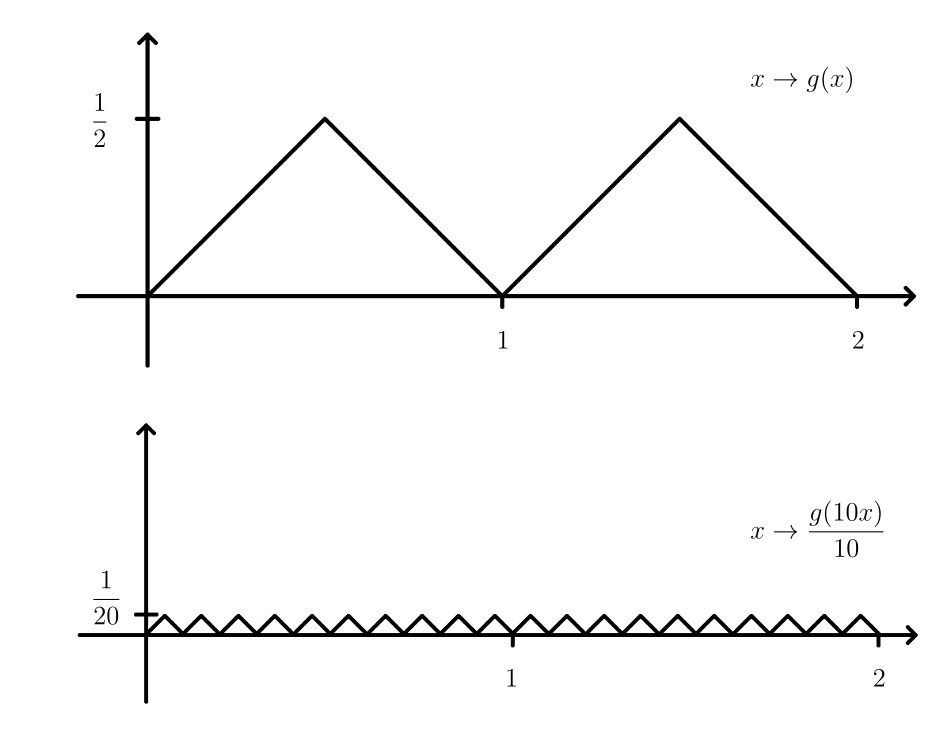
\includegraphics [scale=0.185]{VanDerWaerden.png} \newline
    Sei
    \[ f(x) = \sum_{n=0}^{\infty} \frac{g(10^nx)}{10^n}\]
    Dann ist nach Satz 3.38 diese Reihe auf ganz \( \R\) gleichmässig konvergent und \(f\) ist deswegen stetig. Mittels Dezimalentwicklung kann man zeigen, dass \(f\) in keinem Punkt von \(\R\) differenzierbar ist.
\end{enumerate}
\Def[4.7] \(f: D \rightarrow \R\) ist \textbf{in D differenzierbar}, falls für jeden Häufungspunkt \(x_0 \in D, f\) in \(x_0\) differenzierbar ist. \newline
\Bsp[4.8]
\begin{enumerate}
    \item \( \exp : \R \rightarrow \R \) ist in \( \R\) differenzierbar und \(exp' = exp\)
    Seien \(x_0 \in \R\) und \( h \neq 0:\)
    \[\frac{\exp(x_0 + h)-\exp(x_0)}{h} = \] \newline
    \[\frac{\exp(x_0)\exp(h)-\exp(x_0)}{h} = \] \newline
    \[\exp(x_0) \left[ \frac{\exp(h)-1}{h}\right]\]
    Also: \[ \exp'(x_0) = \exp(x_0) \lim_{h \rightarrow 0} \left[ \frac{\exp(h) - 1}{h}\right]\]
    Aus \( \exp(h) = 1 + h + \frac{h^2}{2!}+ \dots \) folgt für \( h \neq 0\):
    \[\frac{\exp(h) - 1}{h} = 1 + \frac{h}{2!} + \frac{h^2}{3!} + \dots\]
    und für \( h \in [-1,1], h \neq 0\):
    \[ \abs{\frac{\exp(h) - 1}{h}-1} \leq \abs{h} \left[ \frac{1}{2!} + \frac{\abs{h}}{3!} + \dots \right] \leq 2\abs{h}\]
    woraus
    \[ \lim_{h \rightarrow 0} \left( \frac{\exp(h) - 1}{h}\right) - 1 = 0\]
    folgt.
    \item \(\sin' = \cos und \cos' = -\sin\)
\end{enumerate}
\Satz[4.9] Sei \(D \subseteq \R, x_0 \in D\) ein Häufungspunkt von D und \(f,g : D \rightarrow \R \) in \(x_0\) differenzierbar. Dann gelten
\begin{enumerate}
    \item [1] \(f + g\) ist in \(x_0 \) differenzierbar und
    \[(f + g)'(x_0) = f'(x_0) + g'(x_0)\]
    \item [2] \(f \cdot g\) ist in \(x_0\) differenzierbar und
    \( (f \cdot g)'(x_0) = f'(x_0)g(x_0) + f(x_0)g'(x_0)\)
    \item [3] Falls \(g(x_0) \neq 0 \) ist \( \frac{f}{g}\) in \(x_0\) differenzierbar und
    \[ \left(\frac{f}{g}\right)'(x_0) = \frac{f'(x_0)g(x_0) - f(x_0)g'(x_0)}{g(x_0)^2}\]
\end{enumerate}
\Def{} Eine Funktion \(f: \R \rightarrow \R \) heisst \newline \textbf{gerade(resp. ungerade)}, falls \( f(-x) = f(x)\) \newline (resp. \(f(-x) = -f(x)\)) gilt für alle \( x \in \R\) \newline
\Bsp[4.10]
\begin{enumerate}
    \item \( n \geq 1: (x^n)' = nx^{n-1} \quad \forall x \in \R\)
    \item Die Tangensfunktion
    \[ \tan x = \frac{\sin x }{\cos x}, x \notin \frac{ \pi}{2} + \pi \Z\]
    ist auf ihrem Definitonsbereich differenzierbar und
    \[ \tan'(x) = \frac{1}{\cos^2(x)}\]
    \item Die Cotangensfunktion
    \[\cot x = \frac{\cos x}{\sin x}, x \notin \pi \Z\]
    ist auf ihrem Definitonsbereich differenzierbar und
    \[ cot'(x) = -\frac{1}{\sin^2(x)}\]
\end{enumerate}
\Satz[4.11] Seien \(D,E \subseteq \R\) und sei \(x_0 \in D\) ein Häufungspunkt. Sei \(f: D \rightarrow E\) eine in \(x_0\) differenzierbare Funktion so dass \(y_0 := f(x_0)\) ein Häufungspunkt von E ist, und sei \(g : E \rightarrow \R \) eine in \(y_0\) differenzierbare Funktion. Dann ist \(g \circ f : D \rightarrow \R \) in \(x_0\) differenzierbar und
\[ (g \circ f)'(x_0) = g'(f(x_0))f'(x_0)\]
\Korollar[4.12] Sei \(f : D \rightarrow E \) eine bijektive Funktion, \(x_0 \in D\) ein Häufungspunkt; wir nehem an \(f\) ist in \(x_0\) differenzierbar und \(f'(x) \neq 0\) ; zudem nehemn wir an \(f^{-1}\) ist in \(y_0 = f(x_0)\) stetig. Dann ist \(y_0\) Häufungspunkt von E, \(f^{-1}\) ist in \(y_0\) differenzierbar und
\[\left(f^{-1}\right)(y_0)= \frac{1}{f'(x_0)}\]
\newline \newline \newline \newline
\Bsp[4.13] \begin{enumerate}
    \item Die Ableitung von \(\ln : ]0, +\infty [ \rightarrow \R\) ist
    \[ \ln'(x) = \frac{1}{x}\]
    Für alle \(x \in \R \) gilt:
    \[ \ln(\exp(x)) = x\]
    S4.11 für \(f(x) = \exp x\) und \(g(y) = \ln y\)
    \[ \ln'(\exp x)\exp'(x) = 1 \quad \forall x \in \R\]
    und da \( \exp: \R \rightarrow ]0,\infty[\) bijektiv ist, folgt:
    \[ \forall y \in ]0,\infty[: \quad \ln'(y) \cdot y = 1\]
\end{enumerate}
\sep
\subsection{Erste Ableitung}
\Def[4.14] Sei \(f: D \rightarrow \R, D \subseteq \R \) und \(x_0 \in D\)
\begin{enumerate}
    \item [1] f besitzt ein lokales Maximum in \(x_0\) falls es \( \delta > 0 \) gibt mit:
    \[f(x) \leq f(x_0) \quad \forall x \in ]x_0 - \delta, x_0 + \delta [ \cap D\]
    \item [2] f besitzt ein lokales Minimum in \(x_0\) falls es \( \delta > 0 \) gibt mit:
    \[f(x) \geq f(x_0) \quad \forall x \in ]x_0 - \delta, x_0 + \delta[ \cap D\]
    \item [3] f besitzt ein lokales Extremum in \(x_0\) falls es entweder ein lokales Minimum oder Maximum von f ist.
\end{enumerate}
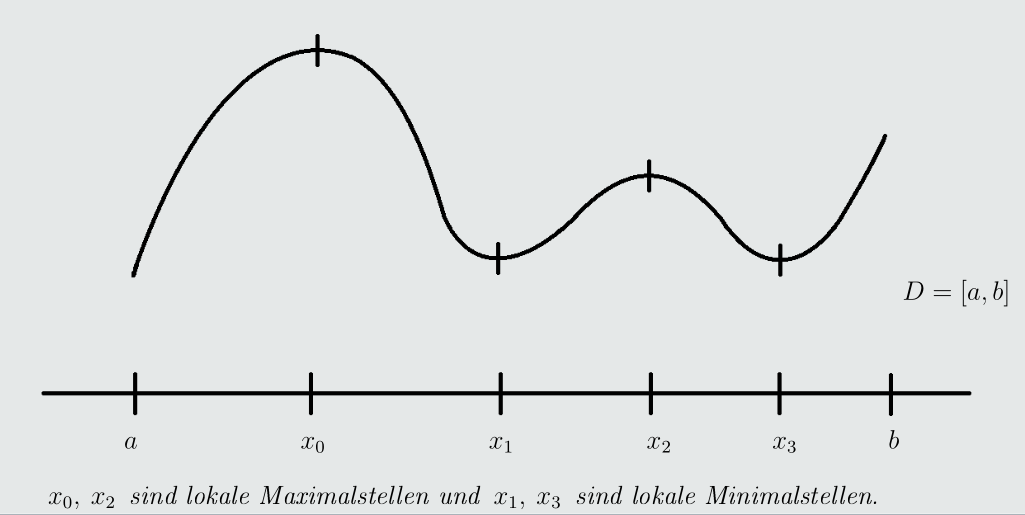
\includegraphics[scale=0.180]{MaximaMinima.png}
\Satz[4.15] Sei \(f: ]a,b[ \rightarrow \R, x_0 \in ]a,b[\). Wir nehmen an, f ist in \(x_0\) differenzierbar
\begin{enumerate}
    \item [1] Falls \(f'(x) > 0\) gibt es \( \delta > 0\) mit
    \[f(x) > f(x_0) \quad \forall x \in ]x_0,x_0 + \delta [\]
    \[f(x) < f(x_0) \quad \forall x \in ]x_0 - \delta ,x_0[\]
    \item [2] Falls \(f'(x_0) < 0 \) gibt es \( \delta > 0\) mit
    \[f(x) < f(x_0) \quad \forall x \in ]x_0,x_0 + \delta [\]
    \[f(x) > f(x_0) \quad \forall x \in ]x_0 - \delta ,x_0[\]
    \item [3] Falls f in \(x_0\) ein lokales Extremum besitzt, folgt \(f'(x_0) = 0\)
\end{enumerate}
\Satz[4.16] (Rolle 1690). Sei \(f: [a,b] \rightarrow \R \) stetig und in \(]a,b[\) differenzierbar. Erfüllt sie \(f(a) = f(b)\) so gibt es \(\mathcal{E} \in ]a,b[\) mit 
\[f'(\mathcal{E}) = 0\]
\hspace*{-3mm}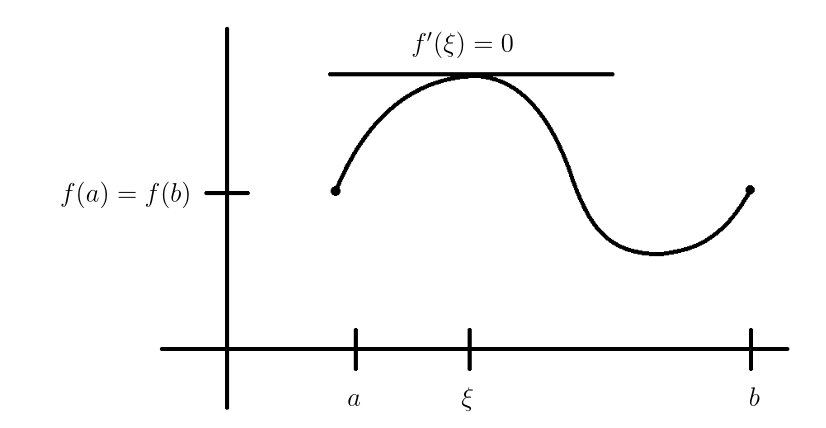
\includegraphics[scale=0.255]{SatzVonRolle.png}
\Satz[4.17] (Lagrange 1797) Sei \(f : [a.b] \rightarrow \R \) stetig mit f in \(]a,b[\) differenzierbar. Dann gibt es \( \mathcal{E} \in ]a,b[ \) mit 
\[f(b) - f(a) = f'(\mathcal{E})(b-a)\]
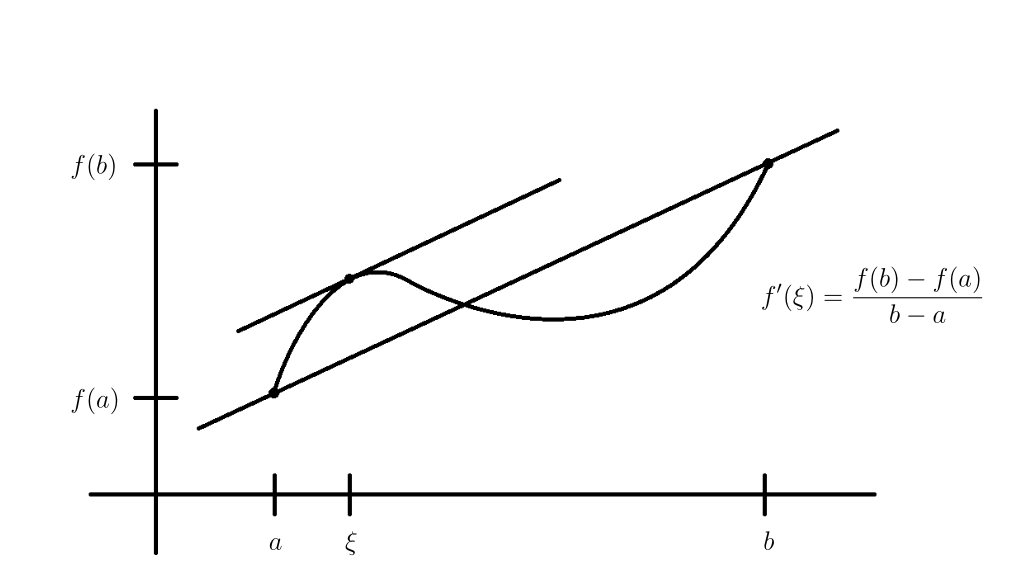
\includegraphics[scale=0.200]{Lagrange.png}
\Korollar[4.18] Seien \(f,g : [a,b] \rightarrow \R\) stetig und in \(]a,b[\) differenzierbar
\begin{enumerate}
    \item [1] Falls \[f'(\mathcal{E}) = 0 \quad \forall \mathcal{E} \in ]a,b[ \  \text{ist f konstant}\]
    \item [2] Falls \(f'(\mathcal{E}) = g'(\mathcal{E}) \quad \forall \mathcal{E} \in ]a,b[ \\ \text{gibt es c} \in \R \text{ mit} f(x) = g(x) + c \quad \forall x \in [a,b].\)
    \item [3] Falls \(f'(\mathcal{E}) \geq 0 \quad \forall \mathcal{E} \in ]a,b[ \\ \text{ist f auf } [a,b] \text{monoton wachsend}\)
    \item [4] Falls \(f'(\mathcal{E}) > 0 \quad \forall \mathcal{E} \in ]a,b[ \\ \text{ist f auf} [a,b] \text{ strikt monoton wachsend}\)
    \item [5] Falls \(f'(\mathcal{E}) \leq 0 \quad \forall \mathcal{E} \in ]a,b[ \\\text{ ist f auf } [a,b] \text{monoton fallend}\)
    \item [6] Falls \(f'(\mathcal{E}) < 0 \quad \forall \mathcal{E} \in ]a,b[ \\ \text{ist f auf } [a,b] \text{strikt monoton fallend}\)
    \item [7] Falls es \(M \geq 0 \) gibt mit
    \[\abs{f'(\mathcal{E})} \leq M \quad \forall \mathcal{E} \in ]a,b[\]
    dann folgt \( \forall x_1, x_2 \in [a,b] : \)
    \[\abs{f(x_1) - f(x_2)} \leq M \abs{x_1 - x_2}\]
\end{enumerate}
\Satz[4.22] (Cauchy). Seien \(f,g : [a,b] \rightarrow \R \) stetig und in \(]a,b[\) differenzierbar. Dann gibt es \( \mathcal{E} \in ]a.b[ \) mit 
\[ g'(\mathcal{E}) (f(b) - f(a)) = f'(\mathcal{E}) (g(b) - g(a))\]
Falls \(g'(x) \neq 0 \quad \forall x \in ]a,b[ \) folgt
\[g(a) \neq g(b)\]
und
\[\frac{f(b) - f(a)}{g(b) - g(a) } = \frac{f'(\mathcal{E})}{g'(\mathcal{E})}\]
Randnotiz: Man erhält den Satz von Lagrange mit \(g(x) = x\) \newline
\Satz[4.23] (l'Hospital 1696) Seien \(f,g : ]a,b[ \rightarrow \R \) differenzierbar mit \(g'(x) \neq 0 \quad \forall x \in ]a,b[\)\newline Falls
\[ \lim\limits_{x \rightarrow b^-}f(x) = 0, \lim\limits_{x \rightarrow b^-} g(x) = 0\]
und
\[ \lim\limits_{x \rightarrow b^-} \frac{f'(x)}{g'(x)} =: \lambda\]
existiert, folgt
\[ \lim\limits_{x \rightarrow b^-} \frac{f(x)}{g(x)} = \lim\limits_{x \rightarrow b^-} \frac{f'(x)}{g'(x)}\]
\Bem{4.24} Der Satz gilt auch 
\begin{enumerate}
    \item [$\bullet$] falls \(b = + \infty\)
    \item [$\bullet$] falls \( \lambda = + \infty\)
    \item [$\bullet$] falls \( x \rightarrow a^{+}\)
\end{enumerate}
\Bsp[4.25]
\begin{enumerate}
    \item Für \( a > 0\) folgt aus S4.13 (1), (2) und l'Hospital:
    \[ \lim_{x \rightarrow \infty} \frac{\ln x }{x^a} = \lim_{x \rightarrow \infty} \frac{\left( \frac{1}{x}\right)}{ax^{a-1}} = \lim_{x \rightarrow \infty} \frac{1}{ax^a} = 0\]
    \item \[ \lim_{x \rightarrow 0^+} x \cdot \ln x = \lim_{x \rightarrow 0^+} \frac{\ln x }{\left( \frac{1}{x}\right)} = \] 
    \[\lim_{x \rightarrow 0^+} \frac{\frac{1}{x}}{-\frac{1}{x^2}} = \lim_{x \rightarrow 0^+} (-x) = 0\]
\end{enumerate}
\Def[4.26] Sei \(I \subseteq \R \) ein Intervall und \(f: I \rightarrow \R \) eine Funktion.
\begin{enumerate}
    \item [1] f ist \textbf{konvex} (auf I) falls es für alle \newline \(x \leq y, \quad x,y \in I \) und \(\lambda \in [0,1]\) \newline
    \(f(\lambda x + (1 - \lambda)y) \leq \lambda f(x) + (1 - \lambda) f(y)\) gilt
    \item [2] f ist \textbf{streng konvex} falls für alle \newline \(x < y, \quad x,y \in I \) und \( \lambda \in ]0,1[\) \newline
    \(f(\lambda x + (1 - \lambda)y) < \lambda f(x) + (1 - \lambda)f(y)\)
\end{enumerate}
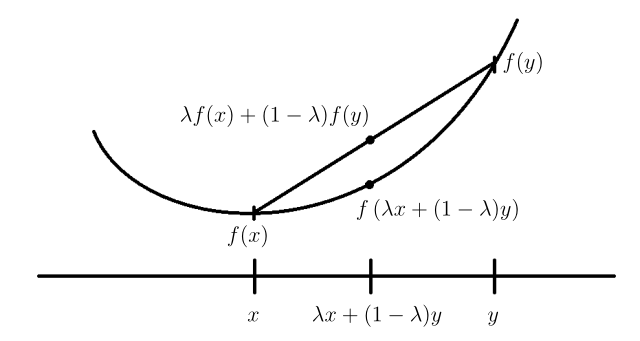
\includegraphics[scale=0.255]{Konvexität.png} \newline
\Bem{4.27} Sei \(f : I \rightarrow \R \) konvex. Ein einfacher Induktionsbeweis zeigt, dass für alle \newline \(n \geq 1, \ \{x_1, \dots x_n \} \subseteq I \) und \(\lambda_1, \dots, \lambda_n\) in \([0,1]\) mit \(\sum_{i=1}^n \lambda_i = 1\)
\[f\left(\sum_{i=1}^n \lambda_i x_i\right) \leq \sum_{i=1}^n \lambda_i f(x_i)\]
\Lemma[4.28] Sei \(f : I \rightarrow \R \) eine beliebige Funktion. Die Funktion f ist genau dann konvex, falls für alle \(x_0 < x < x_1 \) in I
\[ \frac{f(x) - f(x_0)}{x - x_0} \leq \frac{f(x_1) - f(x)}{x_1 - x}\]
gilt.\newline f ist streng konvex wenn \( < \) gilt \newline
\Satz[4.29] Sei \(f : ]a,b[ \rightarrow \R \) in \(]a,b[\) differenzierbar. Die Funktion f ist genau dann (streng) konvex, falls f' (streng) monoton wachsend ist. \newline \newline \newline
\Korollar[4.30] Sei \(f : ]a,b[ \rightarrow \R \) zweimal differenzierbar in \(]a.b[\). Die Funktion f ist (streng) konvex, falls \(f'' \leq 0\) (bzw \(f'' > 0\)) auf \(]a,b[\) \newline
\Bsp[4.31] Für alle \( n \geq 1 \) und \( x_1 \dots x_n\) in \( ]0, \infty [\) gilt
\[ \sqrt[n]{x_1 \dots x_n} \leq \frac{x_1 + \dots + x_n}{n}\]
Wir betrachten \( f(x) = - \ln x\), dann ist
\[ f'(x) = -\frac{1}{x}\]
und
\[ f''(x) = \frac{1}{x^2}, \ x \in ]0,\infty [\]
Folglich ist f konvex und aus Bem. 4.27 mit \newline \( I = ]0,\infty [\) und \( \lambda_1 = \dots = \lambda_n = \frac{1}{n}\) folgt:
\[ -\ln \left( \frac{1}{n} \sum_{i = 1}^{n} x_i\right) \leq \sum_{i=1}^{n} -\frac{1}{n} \ln x_i = -\frac{1}{n} \ln (x_1, \dots x_n)\]
\sep
\subsection{Höhere Ableitungen}
\Def[4.32] Sei \(D \subseteq \R \), so dass jedes \(x_0 \in D \) Häufungspunkt der Menge D ist. Sei \(f : D \rightarrow \R \) differenzierbar in D und f' ihre Ableitung; wir setzen \(f^{(1)} = f'\)
\begin{enumerate}
    \item [1] Für \(n \geq 2\) ist f \textbf{n-mal differenzierbar in D} falls \(f^{(n-1)}\) in D differenzierbar ist. Dann ist \( f^{(n)} := (f^{(n-1)})^{'}\) und nennt sich die n-te Ableitung von f
    \item [2] Die Funktion f ist \textbf{n-mal stetig differenzierbar in D}, falls sie n-mal differenzierbar ist und falls \( f^{(n)}\) in D stetig ist
    \item [3] Die Funktion f ist in D \textbf{glatt}, falls sie \( \forall n \geq 1\), n-mal differenzierbar ist. 
\end{enumerate}
\Bem{4.33} Es folgt aus Korollar 4.5, dass für \(n \geq 1\), eine n-mal differenzierbare Funktion \newline \((n-1)\)-mal differenzierbar ist. \newline
\Satz[4.34] Sei \( D \subseteq \R \) wie in Def. 4.32, \(n \geq 1\) und \( f,g : D \rightarrow \R \) n-mal differenzierbar in D
\begin{enumerate}
    \item [1] \(f+g\) ist n-mal differenzierbar und
    \[(f+g)^{(n)} = f^{(n)} + g^{(n)}\]
    \item [2] \(f \cdot g\) ist n-mal differenzierbar und
    \[(f \cdot g)^{(n)} = \sum_{k=0}^{n} \binom{n}{k} f^{(k)}g^{(n-k)}\]
\end{enumerate}
\Bsp[4.35]
\begin{enumerate}
    \item Die Funktionen \(\exp, \sin, \cos, \sinh, \cosh, \tanh \) sind glatt auf ganz \( \R\)
    \item Polynome sind auf ganz \( \R \) glatt.
    \item \( \ln : ]0,+\infty [ \rightarrow \R \) ist glatt;
    \[ (\ln)'(x) = \frac{1}{x} = x^{-1}, \ (\ln)''(x) = (-1)x^{-2}, \dots\]
    \[\ln^{(n)}(x) = (-1)^{n-1}(n-1)!x^{-n}, \  n \geq 1\]
\end{enumerate}
\Satz[4.36] Sei \( D \subseteq \R \) wie in Def. 4.32, \( n \geq 1 \) und \(f, g: D \rightarrow \R\) n-mal differenzierbar in D
Falls \(g(x) \neq 0 \quad \forall x \in D\), ist \(\frac{f}{g}\) in D n-mal differenzierbar
\Satz[4.37] Seien \(E,D \subseteq \R \) Teilmengen für die jeder Punkt Häufungspunkt ist. Seien \(f:D \rightarrow E\) und \(g: E \rightarrow \R \) n-mal differenzierbar. Dann ist \( g \circ f\) n-mal differenzierbar und
\[(g \circ f)^{(n)}(x) = \sum_{k=1}^n A_{n,k}(x) (g^{(k)} \circ f) (x)\]
wobei \( A_{n,k}\) ein Polynom in den Funktionen \( f', f^{(2)}, \dots , f^{(n+1-k)}\) ist
\[( g \circ f)' = (g' \circ f) \cdot f'\]
\[(g \circ f)^{(2)} = ( g^{(2)} \circ f)(f')^2 + ( g' \circ f) \cdot f^{(2)}\]
\[(g \circ f)^{(3)} = \]
\[(g^{(3)} \circ f) (f')^3 + 3(g^{(2)} \circ f)f'f^{(2)} + (g' \circ f) f^{(3)}\]

\sep
\subsection{Potenzreihen \& Taylor Approx.}
In diesem Abschnitt zeigen wir, dass grob gesagt, konvergente Potenzreihen glatte Funktionen ergeben. Die Umkehrung gilt im Allgemeinen nicht und wird durch eine schwächere Aussage (Taylor Approximation) ersetzt. \newline
\Satz[4.39] Seien  \(f_n: ]a,b[ \rightarrow \R \) eine Funktionsfolge wobei \(f_n\) einmal in \(]a,b[\) stetig differenzierbar ist \( \forall n \geq 1\). Wir nehemen an, dass sowohl die Folge \((f_n)_{n \geq 1}\) wie \((f'_n)_{n \geq 1}\) gleichmässig in \(]a,b[\) konvergieren (Def. 3.34) mit \(\lim\limits_{n \rightarrow \infty} f_n =: f \) und \(\lim\limits_{n \rightarrow \infty} f'_n =: p \). \newline
Dann ist f stetig differenzierbar und \(f' = p\) \newline
\Satz[4.40] Sei \(\sum_{k=0}^\infty c_kx^k\) eine Potenzreihen mit positivem Konvergenzradius (3.39) \(\rho > 0\). Dann ist
\[f(x) = \sum_{k=0}^\infty c_k(x - x_0)^k\]
auf \(] x_0 - \rho, x_0 + \rho [\) differenzierbar und
\[f'(x) = \sum_{k=1}^\infty kc_k(x - x_0)^{k-1}\]
für alle \( x \in ]x_0 - \rho , x_0 + \rho [\) \newline
\Korollar[4.41] Unter der Voraussetzung von Satz 4.39 ist f auf \(] x_0 - \rho, x_0 + \rho[ \) glatt und
\[f^{(j)}(x) = \sum_{k=j}^\infty c_k \frac{k!}{(k-j)!}(x - x_0)^{k-j}\]
Insbesondere ist
\[c_j = \frac{f^{(j)}(x_0)}{j!}\]
\Bsp[4.42](Cauchy 1823)\newline
Das nicht jede glatte Funktion Summe einer Potenzreihe ist, folgt aus diesem Beispiel
\[f(x)=\left\{\begin{array}{cc}
\exp \left(\frac{-1}{x^{2}}\right) & x \neq 0 \\
0 & x=0
\end{array}\right. \]
Diese Funktion ist auf ganz \( \R \) glatt und \newline \( f^{(k)}(0) = 0 \quad \forall k \geq 0\).
Da andererseits  \newline \( f(x) > 0 \quad \forall x \neq 0\), gibt es keine Potenzreihe mit positivem Konvergenzradius \( \rho \), die in \( ]-\rho, \rho [\) gegen f konvergiert. \newline
Aus Satz 4.37 folgt, dass \( \forall k \geq 0\)
\[ f^{(k)}(x) = \mathcal{P}_k \left( \frac{1}{x}\right) \exp \left( \frac{-1}{x^2}\right) \quad \forall x \neq 0\]
wobei \( \mathcal{P}_k\) ein Polynom ist.
Unter Benützung von:
\[ \lim_{x \rightarrow 0} \frac{1}{x^m} \exp \left( \frac{-1}{x^2}\right) = 0 \quad \forall m \geq 0\]
folgt mit \( f^{(k)}(0) = 0:\)
\[ f^{(k+1)}(0) = \lim_{x \rightarrow 0} \frac{f^{k}(x) - f^{(k)}(0)}{x} = \lim_{x \rightarrow 0} \frac{f^{(k)}(x)}{x} = 0\]
\Satz[4.43] Sei \(f: [a,b] \rightarrow \R\) stetig und in \(]a,b[\) \newline (n+1)-mal differenzierbar. Für jedes \(a < x \leq b \) gibt es \(\mathcal{E} \in ]a,x[ \) mit:
\[ f(x) = \sum_{k=0}^n \frac{f^{(k)}(a)}{k!}(x -a)^k + \frac{f^{(n+1)}(\mathcal{E})}{(n+1)!}(x - a)^{n+1} \]
\Korollar[4.44] (Taylor Approximatio)
Sei \(f : [c,d] \rightarrow \R \) stetig und in \(]c,d[ \) (n+1)-mal differenzierbar. Sei \( c < a < d\). Für alle \(x \in [c,d]\) gibt es \( \mathcal{E}\) zwischen x und a so dass
\[f(x) = \sum_{k=0}^n \frac{f^{(k)}(a)}{k!} (x-a)^k + \frac{f^{(n+1)}(\mathcal{E})}{(n+1)} (x-a)^{n+1}\]
Anhand dieses Korollars können wir eine präzisere Aussage über lokale Extremalstellen einer \((n+1)\)-mal differenzierbaren Funktion machen.
\Korollar[4.45] Sei \( n \geq 0,  a < x_0 < b \) und \(f: [a,b] \rightarrow \R\) in \(]a,b[\) (n+1)-mal stetig differenzierbar. Annahme: \(f'(x_0) = f^{(2)}(x_0) = \dots = f^{(n)}(x_0) = 0\)
\begin{enumerate}
    \item [1] Falls n gerade ist und \(x_0\) lokale Extremalstelle, folgt \(f^{(n+1)}(x_0) = 0\)
    \item [2] Falls n ungerade ist und \(f^{(n+1)}(x_0) > 0\) so ist \(x_0\) eine strikt lokale Minimalstelle
    \item [3] Falls n ungerade ist und \(f^{(n+1)}(x_0) < 0\) so ist \(x_0\) eine strikt lokale Maximalstelle
\end{enumerate}
\Korollar[4.46] Sei \(f : [a.b] \rightarrow \R \) stetig und in \(]a,b[\) zweimal stetig differenzierbar. Sei \(x < x_0 < b\). Annahme: \(f'(x) = 0\)
\begin{enumerate}
    \item [1] Falls \(f^{(2)}(x_0) > 0\) ist \(x_0\) strikte lokale Minimalstelle
    \item [2] Falls \(f^{(2)}(x_0) < 0\) ist \(x_0\) strikte lokale Maximalstelle
\end{enumerate}
\Bsp[4.47] Sei \(f(x) = x^4 - x^2 +1\). Wir bestimmen die lokalen Extremalstellen von f. Sei \(x_0\) eine solche; dann folgt nacht Satz 4.15(3):
\[f'(x_0) = 0, \]
das heisst
\[ 4x_0^3 - 2x_0 = 0.\]
Also gilt \(x_0 \in \left\{ -\frac{1}{\sqrt{2}}, 0, \frac{1}{\sqrt{2}}\right\}\). Nun ist \newline \( f^{(2)}(x) = 12x^2 - 2\);
\[ f^{(2)} \left( -\frac{1}{\sqrt{2}}\right) = f^{(2)}\left( \frac{1}{\sqrt{2}}\right) = 4 > 0\]
\[ f^{(2)}(0) = -2 < 0\]
Also sind \( -\frac{1}{\sqrt{2}}\) und \( \frac{1}{\sqrt{2}}\) strikte lokale Minimalstellen, und 0 strikte lokale Maximalstelle.